Description of artificial corruptions.
\begin{table}[H]
    \centering
    \caption{Hyperparameter for different artificial corruption severities}
        \begin{adjustbox}{width=1\textwidth}
            \begin{tabular}{|l||*{11}{c|}}\hline
                \backslashbox{Corruption}{Severity}
                &\makebox[3em]{-5}
                &\makebox[3em]{-4}
                &\makebox[3em]{-3}
                &\makebox[3em]{-2}
                &\makebox[3em]{-1}
                &\makebox[3em]{0}
                &\makebox[3em]{1}
                &\makebox[3em]{2}
                &\makebox[3em]{3}
                &\makebox[3em]{4}
                &\makebox[3em]{5}
                \\\hline\hline
                Defocus blur (radius) &&&&&&0&0.5&1.0&1.5&2&3\\\hline
                Contrast (gain) &3.5&3.0&2.5&2.0&1.5&1&0.9&0.8&0.7&0.5&0.3\\\hline
                Brightness (bias) &-150&-135&-120&-90&-50&0&50&90&120&135&150\\\hline
            \end{tabular}
        \end{adjustbox}
\end{table}

\begin{figure}[H]
	\begin{center}
		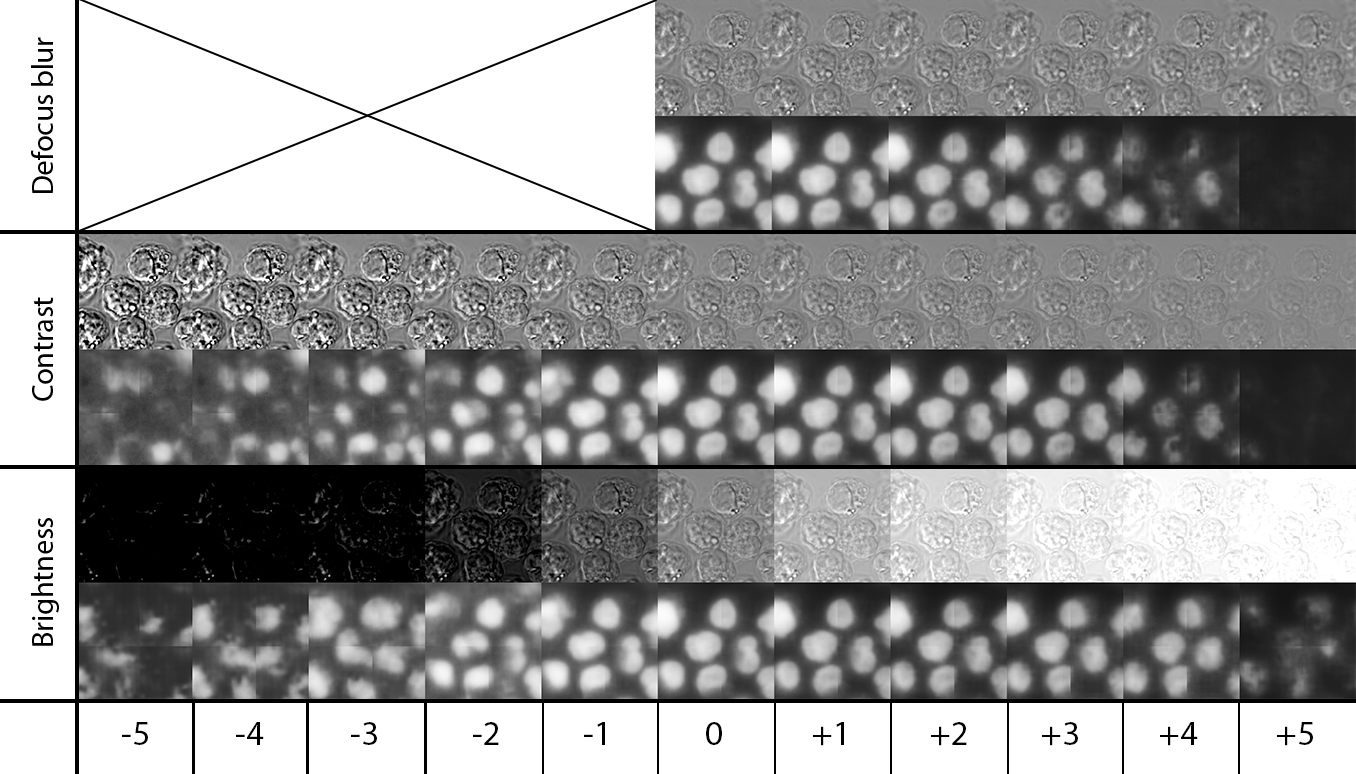
\includegraphics[width=0.5\linewidth]{bilder/corruptions.png}
		\caption{Influence of artificial corruptions on the predictions}\label{fig:artificial-corruptions}
	\end{center}
\end{figure}

\begin{figure}[H]
	\begin{center}
		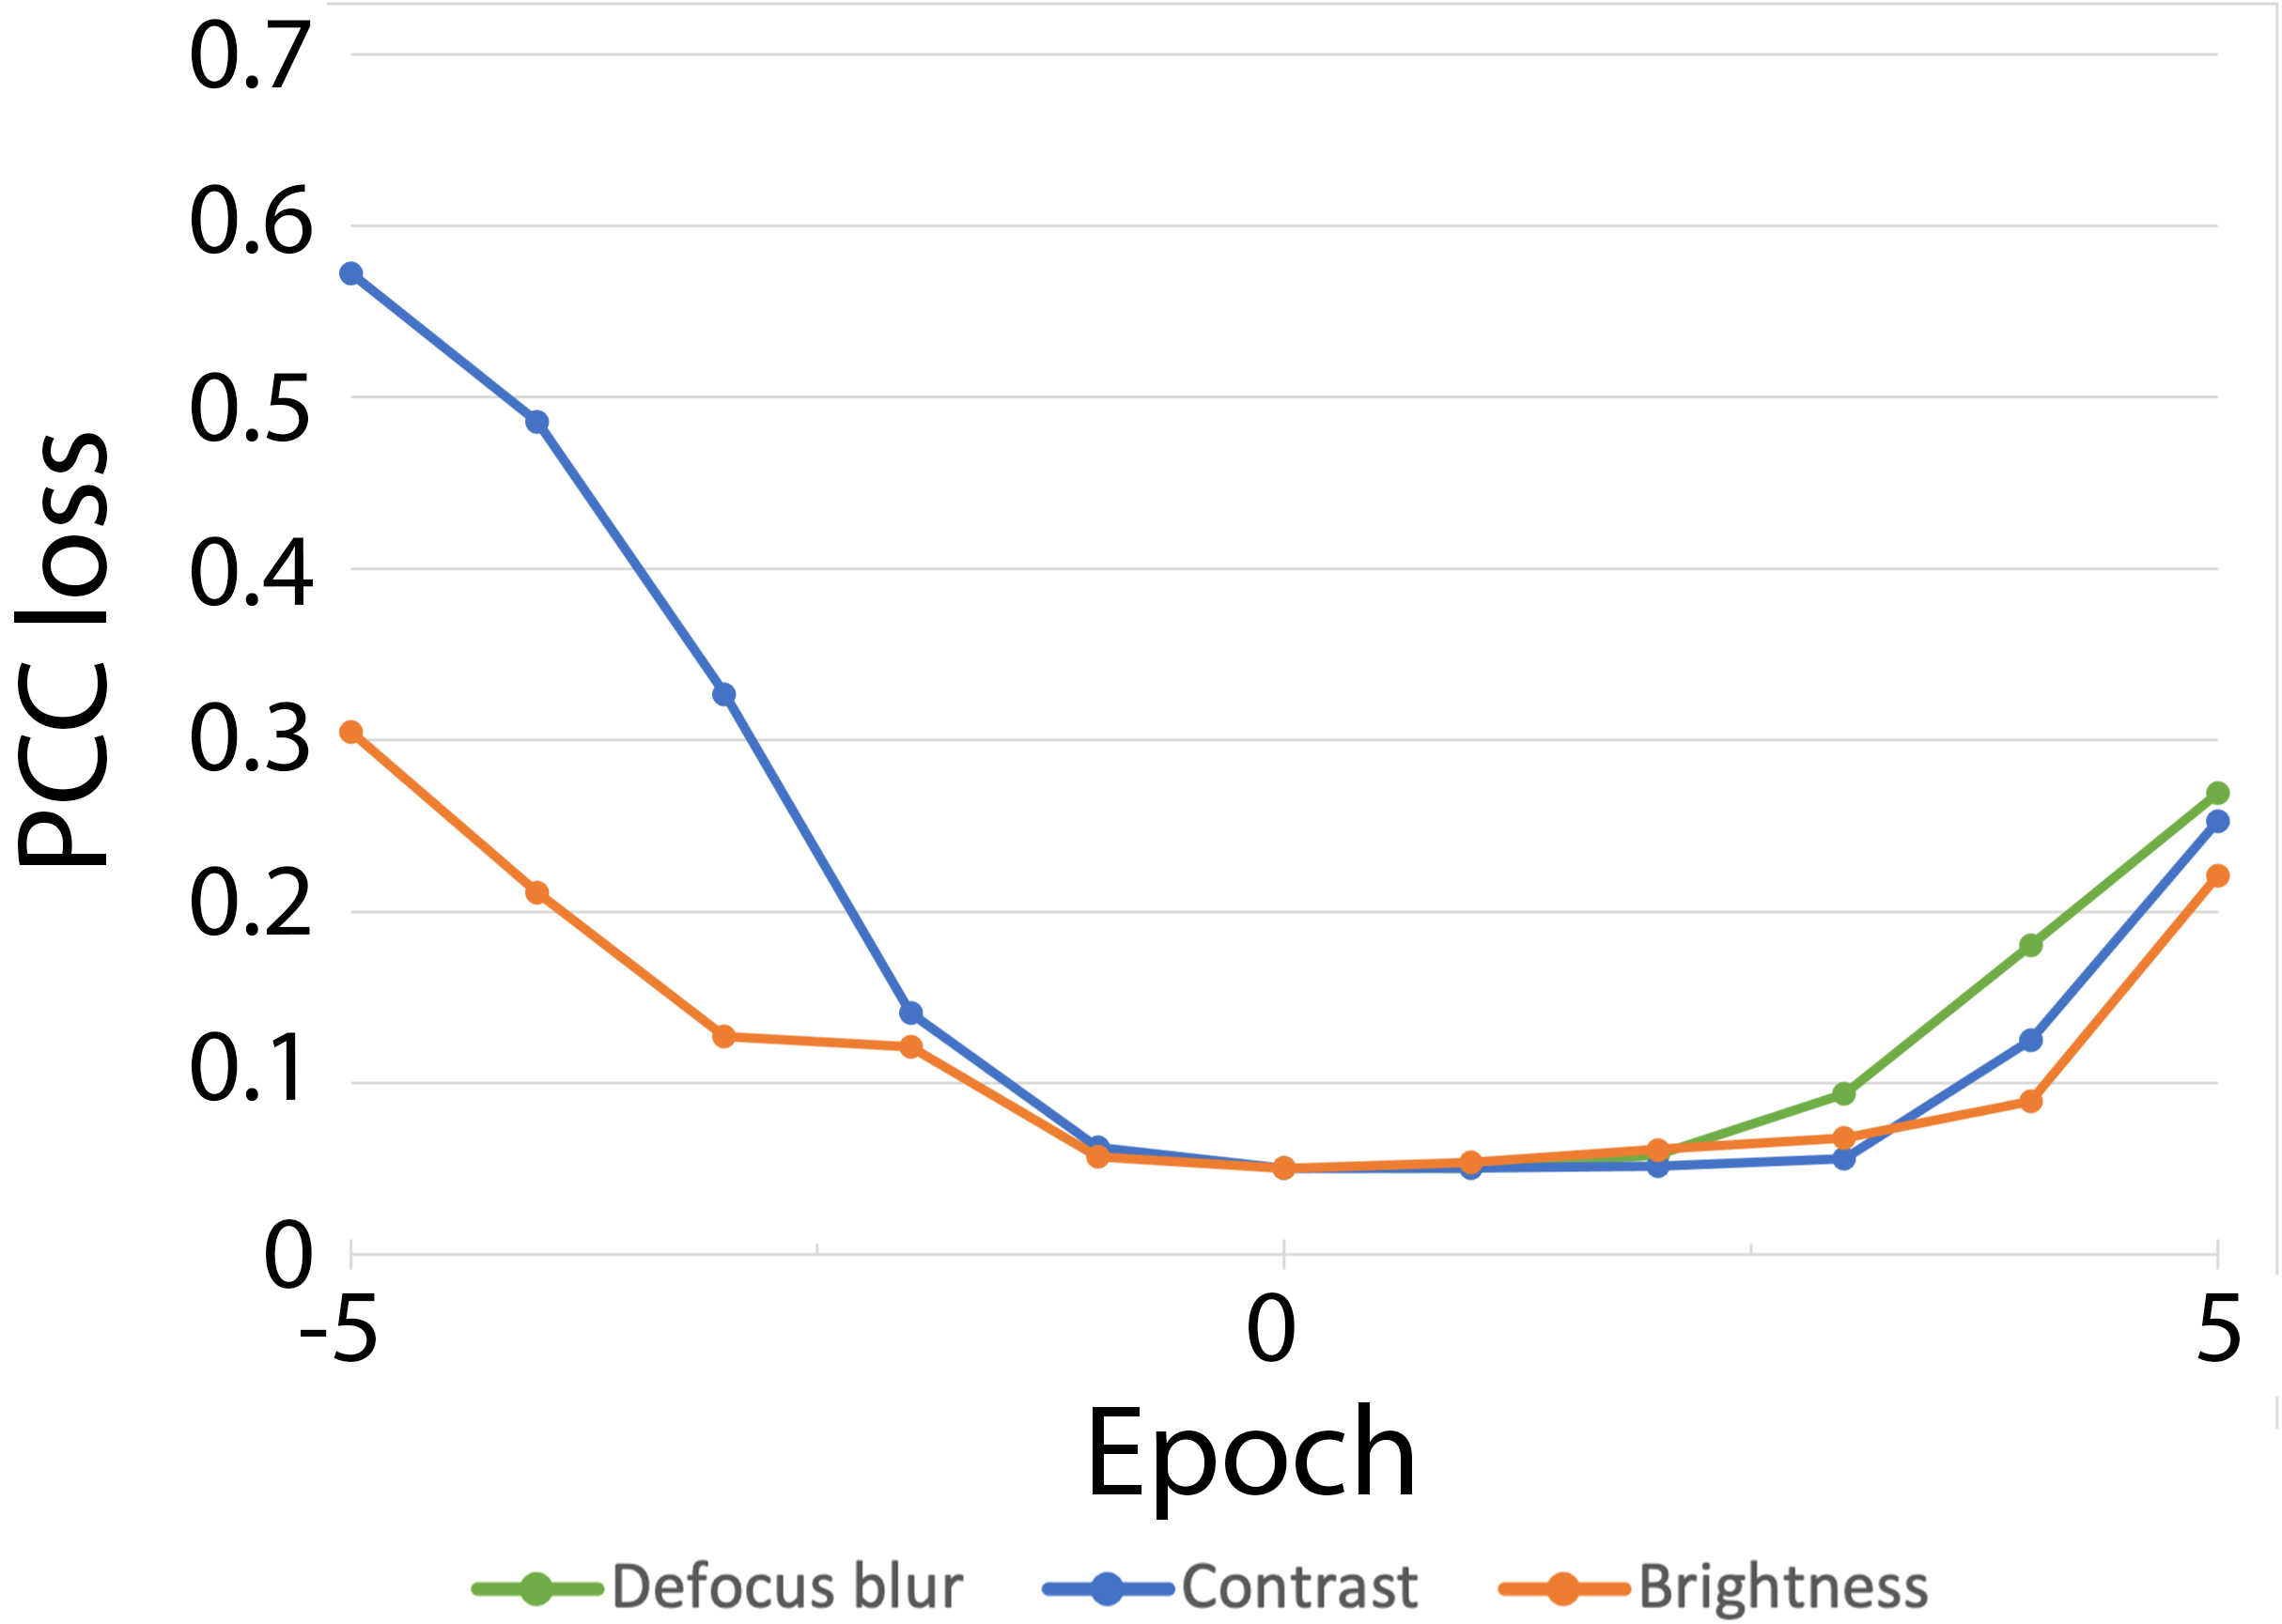
\includegraphics[width=0.5\linewidth]{bilder/corruptions-loss.png}
		\caption{Change of loss for artificial corruptions}\label{fig:corruptions-loss}
	\end{center}
\end{figure}